\section{Evaluation Methodology}

%\subsection{Evaluation Methodology}
Our experiments aim to answer two main questions:
(1) is it possible to model the noise in the training data generated through  \DS, even when there is no prior knowledge to guide us?
%(1) can our transition matrix effectively model the noise in the training data generated through  \DS?
% both sentence level and bag level, TM could reduce all three levels, by masking the TM, for NA related relations.
%(2) can we estimate the transition matrix if there is no prior knowledge to guide us?
% can we better handle those noise in different situations?
%
and (2) whether the prior knowledge of data quality can help our approach better handle the noise.

We apply our approach to both sentence level and bag level
extraction models, and evaluate in the situations where prior knowledge of
the data quality is available as well as the situation where such prior
knowledge is missing.


%We show that our method works in all of these settings and prior knowledge of the data quality can benefit the training of transition matrix. We also find that the sentence level models works better when we have both reliable and unreliable data, but the bag level model performs better if all the data are treated equally. Furthermore, to explore the generalization ability of our method, we also conduct experiments in two datasets.
\subsection{Datasets}
We evaluate our approach on two datasets. The first one is  \TimeRE, constructed by ourself using \DS.
 It is used to evaluate our approach on scenarios with and without prior knowledge about the
data quality. The second dataset is the widely used \EntityRE dataset~\cite{riedel2010modeling},
which provides no prior knowledge of the data quality.


\paragraph{\TimeRE}
 is automatically constructed by using \DS to align time-related Wikidata\cite{vrandevcic2014wikidata} knowledge triples to
Wikipedia text, containing 278,141 sentences with 12
types of relations  between an entity mention and a time expression.
We choose time-related relations in this dataset as time expressions speak for themselves in
terms of reliability. That is, given a knowledge triple $<$$e,rel,t$$>$ and its
aligned sentences,  the  finer-grained the time expression $t$ appears in the sentence,
the more likely the sentence  supports the existence of this triple.
For example, a sentence containing both \texttt{Alphabet} and \texttt{October\_2\_2015} is highly likely to express the \texttt{inception-time} of \texttt{Alphabet}, while a sentence containing both \texttt{Alphabet} and \texttt{2015} could instead talk  about many events, e.g.,  releasing financial report of 2015, hiring a new CEO, etc.
Using this heuristics, we split the dataset into
3 subsets according to different granularities of the time expressions involved, indicating different levels of reliability.
Our criteria for determining the reliability of the data are as follows.
Instances with full date expressions, i.e., \texttt{Year-Month-Day}, can be seen as the most reliable data, while those with
partial date expressions, e.g., \texttt{Month-Year} and \texttt{Year-Only}, can be seen as less
reliable.  Negative data are constructed  heuristically that any
\emph{entity-time} pairs in a sentence without corresponding triples in Wikidata are considered as negative data.
%\red{we still have noises in terms of \textbf{false negative}, right? do we have experiments to say this? } \orange{yes, but no experiments}
During training, we can access  184,579 negative
instances and  77,777 positive instances, including 22,214 reliable
ones, 2,094 and 53,469 less reliable ones. The validation set and test set are randomly sampled from
the reliable (full-date) data for relatively fair evaluations and contains
2,776, 2,771 positive instances and 5,143, 5,095 negative instances, respectively.
%\red{talk bag level numbers?????} \orange{maybe too messy? how about only showing sentence level numbers in both dataset?}


\paragraph{\EntityRE} is a widely-used entity
relation extraction dataset, built %by independent researchers
by aligning triples
in Freebase to the New York Times (\NYT) corpus~\cite{riedel2010modeling}. It contains 52 relations, 136,947 positive and 385,664 negative sentences for training, and 6,444 positive and 166,004 negative sentences  for testing.
Unlike \TimeRE, this dataset does not contain any prior knowledge about the data quality.
However, it is a good example to evaluate the generalization ability of our transition matrix approach.
\emph{Since the sentence level annotations in the test set of \EntityRE are too noisy to serve as gold standard,  we only evaluate bag-level models on \EntityRE -- a standard practice in previous works}~\cite{surdeanu2012multi,zeng2015distant,lin2016neural}.


\begin{figure}[t!]
\begin{center}
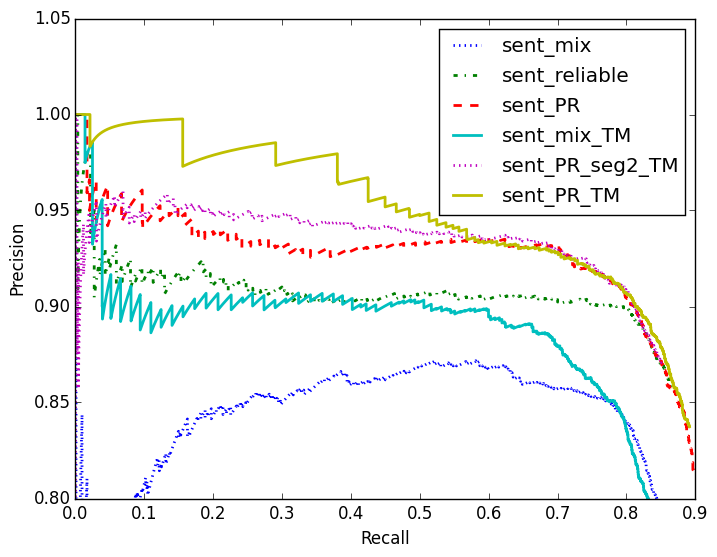
\includegraphics[width=0.9\linewidth]{figures/sent_time_exp_overall.png}
\caption{Sentence Level Results on TimeRE}
\label{fig: sent_luo}
\end{center}
\end{figure}

%\subsection{Experimental Setup}

\subsection{Hyperparameters}

\paragraph{Neural network components} used in our algorithm are based on a convolution neural network with 200 convolution kernels and the window size is 3. To train the network, we use stochastic gradient descend (SGD) with a batch size of 20.  The learning rates for sentence-level  and bag-level models are 0.1 and 0.01, respectively.

\paragraph{Sentence level modeling}
 is performed on the \TimeRE dataset, where we use 100-dimensional word embeddings pre-trained using GloVe~\cite{pennington2014glove} on Wikipedia and Gigaword\footnote{\url{catalog.ldc.upenn.edu/LDC2011T07}}, and 20-dimensional vectors for distance embeddings. Each of the three subsets of \TimeRE is added after the previous phase has run for 15 epochs. \blue{The trace regularization weights for the three subsets are $\beta_1=0.01$, $\beta_2=-0.01$ and $\beta_3=-0.1$, respectively, from the reliable to the most unreliable part, and the ratio of $\beta_3$ and $\beta_2$ is fixed to 10 or 5 during hyper-parameter tuning.}

\paragraph{Bag level modeling}
is performed on both  \TimeRE and  \EntityRE datasets. We use the same parameters as sentence level for \TimeRE.
%The parameters of the bag level model is almost the same as the sentence level model on TimeRE data, except that the learning rate is 0.01 and the less reliable data are added when the previous phase has run for 3 and 6 epochs.
For \EntityRE, we use 50-dimensional word embeddings pre-trained on the \NYT corpus using word2vec\footnote{\url{code.google.com/p/word2vec/}}. The size for distance embedding is 5. For both datasets, the linear combination parameter $\alpha$ is 1 and the trace regularization parameter $\beta$ is initialized to 0.1. We tried various decay rates, \{0.95, 0.9, 0.8\}, and decay steps, \{3, 5, 8\}. We found that using a decay rate of 0.9 and step of 5 gives best performance in most cases.

\subsection{Evaluation Metric}
The performance is reported using the precision-recall (\PR) curve, calculated according to the extraction results ranked decreasingly by their confidence scores. This is a standard evaluation metric in relation extraction.

\subsection{Naming Conventions}
We evaluate our approach under a wide range of settings for
 sentence level
(\texttt{sent\_}) and bag level (\texttt{bag\_}) models:
(1) \texttt{\_mix}: models are trained on the three subsets of \TimeRE mixed together;
(2) \texttt{\_reliable}: models are trained using the reliable subset of \TimeRE only;
(3) \texttt{\_PR}: models are trained with prior knowledge of annotation quality, i.e., starting from the reliable data and then adding the unreliable data;
(4) \texttt{\_TM}: models are trained with dynamic transition matrix;
(5) \texttt{\_GTM}: models are trained with a global transition matrix;

%\footnote{Since curriculum learning without prior knowledge is our default training method, we use \texttt{\_CL} to refer to the situation with prior knowledge of data quality here for simplicity. \red{ZW: What???}}.

For bag level modeling, we also evaluate the model performance using average aggregation (\texttt{\_avg})
and attention aggregation (\texttt{\_att}), as described in Section~\ref{sec:baglevelmodeling}.

\begin{figure*}[htbp]
\centering
\subfigure[Attention Aggregation]{
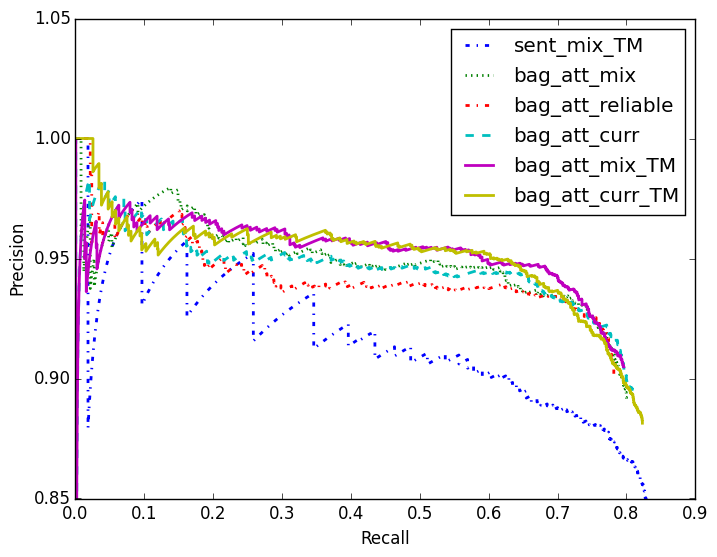
\includegraphics[width=0.45\linewidth]{figures/bag_att_exp_overall.png}
\label{fig: bag_att_luo}
}
\subfigure[Average Aggregation]{
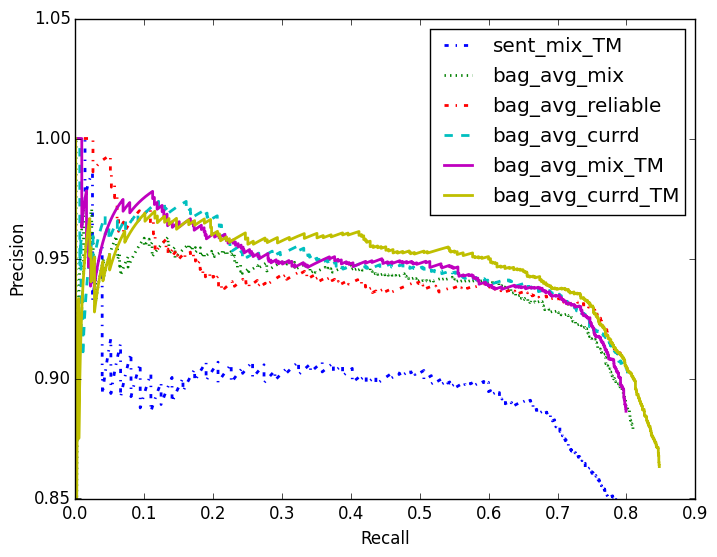
\includegraphics[width=0.45\linewidth]{figures/bag_avg_exp_overall.png}
\label{fig: bag_avg_luo}
}
\caption{Bag Level Results on TimeRE}
\label{fig: results_on_luo}
\end{figure*}

